\documentclass{article}
\usepackage{graphicx}
%\usepackage{varwidth}
%\usepackage{caption}
%\usepackage{float}
\usepackage{picinpar}
\begin{document}
%	\begin{figure}[ht]
%		
\includegraphics[scale=0.4]{snuggle.jpg}
%		\caption{in plain format, if title too long, like normal paragraphics for display. 
%		if you set the formal small title,you can cut for paragraphics}
%	\end{figure}\par

%	\begin{table}
%		\begin{tabular}{c|c|c}
%			name & sex & grade\\
%			\hline
%			lily & female & 6\\
%			lucy & female & 4\\
%			peter & male & 6\\
%		\end{tabular}
%		\caption{student information}
%	\end{table}\par

%\begin{figure}
%	
\includegraphics{snuggle}
%	\includegraphics{number}
%	\caption{this is picture}
%\end{figure}

%\begin{figure}
%	\subfigure[caption_01]{
%		
\includegraphics[scale=0.4]{snuggle}
%	}
%	\subfigure[caption_02]{
%		\includegraphics[scale=0.4]{nuber}
%	}

%	\begin{figure}
%		\centering
%		\begin{varwidth}[t]{\textwidth}
%			\vspace{0pt}
%			
\includegraphics[scale=0.2]{snuggle.jpg}
%		\end{varwidth}
%		\begin{varwidth}[t]{\textwidth}
%			\vspace{0pt}
%			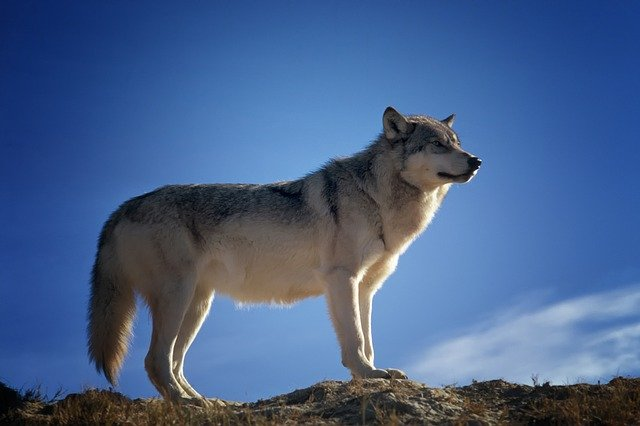
\includegraphics[scale=0.2]{wolf.jpg}
%		\end{varwidth}
%	\end{figure}

\begin{figwindow}[2,l,
	{
\includegraphics[width=8cm]{snuggle.jpg}},Lion]
	Alice was beginning to get very tired of sitting by her sister on the bank, and of having nothing to do: once or twice she had peeped into the book her sister was reading, but it had no pictures or conversations in it, ‘and what is the use of a book,’ thought Alice ‘without pictures or conversations?’

So she was considering in her own mind (as well as she could, for the hot day made her feel very sleepy and stupid), whether the pleasure of making a daisy-chain would be worth the trouble of getting up and picking the daisies, when suddenly a White Rabbit with pink eyes ran close by her.

In another moment down went Alice after it, never once considering how in the world she was to get out again.

The rabbit-hole went straight on like a tunnel for some way, and then dipped suddenly down, so suddenly that Alice had not a moment to think about stopping herself before she found herself falling down a very deep well.
\end{figwindow}

\end{document}


% begin{figure}[]...\end{figure}用于图片浮动体

% begin{table}[]...\end{table}用于表格浮动体

% table和figure环境共同可选参数列表:
% h - 浮动体根据上下文顺序排列
% t - 浮动体排在当前页或下一页页首
% b - 浮动体排在当前页页尾
% p - 浮动体另外一页进行排列
% H - 不适用浮动体,不能与其他选项合用。包含在float宏包中
% 参数的优先级与顺序无关,通常按htbp顺序排列;当只有h参数时,拓展为ht参数集合;默认参数集合为tbp

% LaTeX最多同时保存18个未处理的浮动体

% \caption{string}为浮动体中的标题。并且有两种类型:
% 1.\caption{<title>}
% 2.\caption{<short_title>}{<long_title>},long_title可进行分段

% 将多个表格/图标盒子在同一个浮动体中,可以并列排放。其中,表格按垂直方向居中对其,图片按垂直方向的基准线对齐

% \subfigure用于单个浮动体内的多个图像,分别标注标题。包含在subfigure宏包中

% \begin{varwidth}[t]{\textwidth}...\end{varwidth}用于确定宽度;\vspace{0pt}用于配置一个0pt空行,并按空行进行对齐,即top对齐。该功能包含在varwidth宏包中
 
 % \begin{figwindow}[下降行数, 水平位置, 图内容, 图表题]...\end{figwindow}用于指定图片四周的文字绕排。包含在picinpar宏包中
 
 
 